section{methods}

\pagestyle{plain}

subsection{Measurement}

TEM measurement includes sample preparation. It is very important to have
the sample dry during the TEM measurement so the preparation must start
a few hours before. The very first step is getting the copper grids with carbon
coating. The reason for using copper grid is its conductivity, so the electrons
from the TEM can go thru the grid easily and it also is not so expensive like gold
or platinum girds. In the second step it is necessary to adsorb the solution that is
to be measured onto the grid. The volume of pipetted solution has to be proportional
to the size of the grid. After that the samples have to become dry.
That is the reason why it was prepared several hours before the measurement.
The samples are being prepared using dropcasting, pipette with volume 1 μL was used.

\begin{figure}[h]
    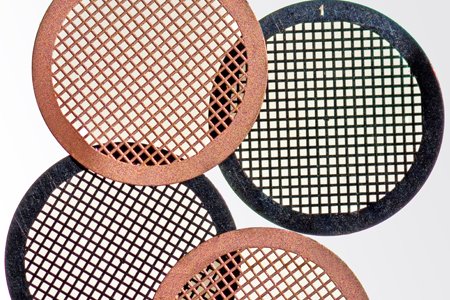
\includegraphics[width=\linewidth]{grid.jpg}
    \caption{Diagram of copper grid, taken from \cite{}}
    \label{fig:otsu}
\end{figure}

The microscope measurement itself is being done by microscope technician.
The measurement begins with putting the grid with the sample into the microscope.
Then it is necessary to focus it on the place where the sample is. It is good to make
more than one picture of each sample. It is also important to find places where are
some particles but where these do not overlap so much.

subsection{Image analysis}

Another step is creating program in image analysis, it is writen in Python.
There were used several Python libraries, most of segmentation methods were
implemented using Scikit image library, there were also used opencv for Python
and Scipy ndimage for some functions, these libraries are using Numpy, which
is library used for work with martices. There was also used Matplotlib Pyplot
library for plotting and saving images.

First step after loading TEM image is convering it into grayscale due it could
be filtrated. TEM images can be of different scales and size and number of particles
in image depends on it. Median filter is used for denoising image. Filtrating works
of principle of convolution and size and appearance of convolution mask determine type
of filter. Median filter belongs to nonlinear filters which means that output is not
linear function of input. Median filter simply counts median value from neighborhood
of certain pixel for every pixel in image. Advantage of this filter is that it
preserv edges and removes noise. Size of kernel or pixel neighborhood depends on
scale of input image and also on type of particles because nanords are usually
smaller than nanoparticles so it has to be blured less.

Then grayscale image has to be transform into binary image. It is usually done
by finding appropriate threshold and pixels with value below threshold are 
transformed to zero and pixels with value above threshold are transformed into
one or 255 (it depends if binary image values are of type boolean with just 0 and 1
or 8-bit unsigned integer with values from 0 to 255). In case of this project
binary image is also inverted. In TEM images particles are black on white background
so in binary image particles pixels should be zero and background pixels should be one
and for this application it is better to invert it. There are several types of
thresholding techniques. Theese techniques uses histogram for calculating
appropriate threshold. There were used two different techniques in this project.
Minimum threshold method find pixel valu with minimum frequency in histogram and
this value is determined as threshold. Other method is called Otsu thresholding
and it is a bit more complicated algorithm. It consists in going throught every
pixel value and calculate variance in pixel values below this pixel and above this pixel
and finds pixel value with the smallest variance. This pixel value is determined as
threshold. Otsu thresholding is more advanced method and whould work better, but
in nanoparticles images with larger scale (there were just a few dart particles in center
of image) this method calculated too high threshold. More than just parctiles pixels
were determined as foreground. So it was chosen to use minimum thresholding method for
nanoparticles and Otsu thresholding method for nanorods.

After binarizing image there are used morphology operation to clean up image.
There are two basic operations called erosion and dilation. It works on principle
of interaction with structuring element which determines shape of pixel's neighborhood.
Dilation is used for filling holes and it increases size of objects. Algorithm changes pixel
value to one if there are enought white pixels in its neighborhood. Erosion is opposite
of dilation, it is used for removing small objects and it decreases size of objects.
Algorithm changes pixel value to zero if there are not enought white pixels in its
neighborhood. There are also two methods wchich consist of both erosion and dilation.
Opening first uses erosion and later dilation, it is used for removing small objects.
Closing first uses dilation and later erosion, it is used for removing small holes.
Opening and closing are better because it changes sizes of objects less than just erosion
and dilation. In scikit image library there are also fucntions designed perfectly
for removing small objects or holes. These scikit image function were also used
in this project for removing artifacts from background and fill holes in particles.

Main part of this project is image segmentation which separates particles so it could
be analyzed. There are plenty of methods used for segmentation and it is quite difficult
task to choose the best method and implement it. For this project watershed transformation
was chosen as main method. This algorithm starts with seeds and binary image. Seeds are
points or small clusters of points. In perferct world there should be one seed per
particle in image. Algorithm takes seeds and starts filling binary mask from theese points.
It is called watershed because seeds can be imagined as valleys (or local minima) and
algorithm fills every valley with water of different value starting from local minima.
It ends when it reaches edge of binary mask or when it meets water from another valley.
Labeled image is created, each pixel in one label has same number, background has zero.
There are more methods how to find seeds, in this project method called distance map
was used. It works on principle of finding for each zero pixel distance (number of pixels)
to the closest white pixel. Seeds were created by finding local maxima in distance fucntion.
It may happen that algorithm oversegments image so there are some small artifacts. So it
was decided to filter too small labels. It is done by algorithm which is giong throught
all labels and calculating median of their areas. If area of current labels is smaller
than median divided by 1.5 (number was estimated experimentally), label is removed.
The algorithm finishes when there are no label smaller than median divided by 1.5.

Watershed perfectly divides non-overlapping particles. In overlapping particles may occure
two cases, watershed divided particles well but did not count with their parts which
overlap, or it does not devide particles well so it finds one big label. Due to this
problem it was decided to use also another segmentation method. First ROI (region of
interest) is defined. ROI is defined for every overlapping particles. Each ROI is
croped image wchich contain only these ovelapping particles. Detection of overlapping
particles is done by finding each connected region and its area is compared with
median area of labels. If area of connected object is 1.5 times bigger than median,
it is clasifyed as overlapping particles and ROI of this object is created.
It was decided to perform hough transformation to detect circles in image. Hough
transformation wors on principle of transfering image space into hough space, which means
there are different axis. Hough circle transform takes every point in binary edge image,
considers it is circle edge and finds every potential centers of this edge point.
It means for each x and y in potential circle edge there is function of cx, cy and r,
which describes coordinates of potential circle centers and potential circle radius.
For each radius, there is cirle in hough space for each point in image space and
point in hough space for each circle in image space. Limits of cx and cy are given by
image size, but there is no limitation for radii. So the limitation must be defined
manually. Function in scikit image library calculates cx, cy, r and weight of each
detected circle, it means how detected circle fits to the edges. First step in hough
transformation is performing canny edge detection, which is algorithm containing
high filtrating (marks up edges) and binarizing, so result is binary image with marked
up edges. Theese edges can be used in function for hough transform, hough transform
returns weight, center coordinates and radius for each detected circle. Then the result
has to be filtrated, it may contain more than one detected circle for just one circle in
image or it may detect wrong edges (too small or too big in compare to other circles).
So it is defined minimum distance between two centers and minimum weight of detected circle.
Than median area of all circles is calculated and circles smaller than median divided by
1.5 or circles larger than median multiplicated by 3 (both numbers estimated experimentally)
are removed.

In summary, non-overlapping particles are detected by watershed algorithm and ovelapping
particles by hough transformation. There is also hough transform for ellipse, which could
be used for nanorods but it will be part of following project. In this project nanorods are
detected only by watershed. After it, it is important to calculate particle properties.
For nanoparticles area and diameter is calculated and for nanords area and major axis and
minor axis length.